\documentclass{article}
\usepackage[final]{neurips_2024}
\usepackage[T1]{fontenc}    
\usepackage{hyperref}       
\usepackage{url}            
\usepackage{booktabs}       
\usepackage{amsfonts}       
\usepackage{nicefrac}       
\usepackage{microtype}      
\usepackage{xcolor}         
\usepackage{graphicx}   
\usepackage{amsmath}
\usepackage{float}

\setcitestyle{numbers}

\title{COMP 579 Final Project Report: Reinforcement Learning for Ms. Pac-Man}

\author{
    Ivy Hu\textsuperscript{1} \quad
    Simon Li\textsuperscript{2} \quad
    Kenza Bellebouir\textsuperscript{1} \\
    \texttt{nanqing.hu@mail.mcgill.ca} \quad
    \texttt{xi.yang.li@mcgill.ca} \quad
    \texttt{kenza.bellebouir@mail.mcgill.ca} \\
    \textsuperscript{1}Department of Computer Science, McGill University \\
    \textsuperscript{2}Department of Electrical Engineering, McGill University
}

\begin{document}

\maketitle

\begin{abstract}
  We investigate the comparative performance of Rainbow DQN and Proximal Policy Optimization (PPO) in the visually complex Ms. Pac-Man environment. Our study evaluates learning dynamics, hyperparameter sensitivity, and robustness to visual perturbations. Rainbow DQN consistently achieves higher peak rewards and demonstrates stronger long-term learning, while PPO shows faster early convergence but suffers from instability. We also conduct ablation studies and color-based generalization tests, offering practical insights into the role of architecture and training design in sparse-reward, high-variance domains.
\end{abstract}

\section{Introduction}

Deep reinforcement learning (RL) has achieved notable success in high-dimensional decision-making tasks, particularly within the Arcade Learning Environment (ALE) \cite{ale}, which provides a unified platform for evaluating algorithms on Atari 2600 games \cite{mnih2015human}. These environments are characterized by partial observability, sparse and delayed rewards, and the need for both short-term reactivity and long-term planning.

Among them, \textit{Ms. Pac-Man} is a particularly challenging domain due to its stochastic dynamics, diverse strategic possibilities, and visually rich inputs. It is thus well-suited for evaluating algorithmic robustness and scalability. In this work, we compare two prominent deep RL methods: Rainbow DQN \cite{hessel2018rainbow}, an enhanced value-based agent that integrates six key improvements over DQN, and Proximal Policy Optimization (PPO) \cite{schulman2017proximal}, a widely used policy-gradient algorithm known for its simplicity and stability.

We implement both agents in the \texttt{MsPacman-v0} environment and conduct a detailed empirical evaluation. Beyond comparing baseline performance, we perform an ablation study of Rainbow DQN to assess the contribution of prioritized experience replay, noisy networks, and multi-step returns. To evaluate generalization, we test trained agents under visual domain shifts introduced via color perturbations. We further analyze sensitivity to hyperparameters by conducting targeted sweeps to identify configurations yielding strong and stable performance.

This study provides insights into the design and evaluation of RL algorithms in complex visual settings, highlighting the internal dynamics and generalization capabilities of Rainbow DQN relative to PPO.

\section{Background}

\subsection{Reinforcement Learning and MDPs}

Reinforcement Learning formalizes sequential decision-making as a Markov Decision Process (MDP), defined by $(\mathcal{S}, \mathcal{A}, \mathcal{P}, \mathcal{R}, \gamma)$, where $\mathcal{S}$ is the state space, $\mathcal{A}$ the action space, $\mathcal{P}(s'|s,a)$ the transition model, $\mathcal{R}(s,a)$ the reward function, and $\gamma \in [0,1)$ the discount factor. The agent selects actions to maximize expected return $\mathbb{E}[\sum_t \gamma^t r_t]$ based on its interactions with the environment.

\subsection{The Ms. Pac-Man Environment}

The \texttt{MsPacman-v0} environment is a high-dimensional, partially observable MDP. Each observation is a $210 \times 160 \times 3$ RGB frame, preprocessed to $84 \times 84$ grayscale. The action space consists of discrete directional commands and a no-op. Reward signals are sparse, with +10 for pellets, +200 for ghosts after consuming a power pellet, and a time-step penalty of –1. An episode ends when the agent loses three lives.

This environment presents multiple challenges: pixel-based observations limit access to the full game state, ghost behavior is stochastic and partially unpredictable, and the sparse reward structure complicates credit assignment and learning signal propagation. Additionally, the lack of intermediate rewards increases the difficulty of learning effective threat avoidance or path planning strategies.

\subsection{Rainbow DQN}

Rainbow DQN \cite{hessel2018rainbow} combines several enhancements to the original DQN \cite{mnih2015human}, aiming to improve sample efficiency, stability, and exploration. Double Q-learning addresses overestimation bias by decoupling action selection and evaluation in target computation. The dueling network architecture separates state-value and advantage estimation to refine action selection. Prioritized experience replay focuses learning on high-error transitions, improving data efficiency. Noisy networks inject trainable stochasticity into parameters, facilitating more efficient exploration. Multi-step returns accelerate learning by propagating rewards over multiple future steps. Distributional RL (C51) models a categorical distribution over future returns, enabling richer value representation.

\subsection{Proximal Policy Optimization (PPO)}

PPO \cite{schulman2017proximal} is a first-order policy-gradient algorithm that improves training stability by limiting policy updates through a clipped surrogate objective:
\[
L^{\text{CLIP}}(\theta) = \mathbb{E}_t \left[ \min \left( r_t(\theta) \hat{A}_t, \text{clip}(r_t(\theta), 1 - \epsilon, 1 + \epsilon) \hat{A}_t \right) \right],
\]
where $r_t(\theta)$ is the probability ratio between the new and old policies, and $\hat{A}_t$ is an estimate of the advantage function. PPO strikes a balance between exploration and stability, making it suitable for a wide range of tasks without extensive tuning.

\subsection{Evaluation Challenges}

Evaluating agents in visually rich environments like Ms. Pac-Man is non-trivial. RL training is often unstable due to non-stationarity, bootstrapping errors, and high sensitivity to hyperparameters. Sample efficiency is critical, especially when training from pixel inputs requires millions of frames. Generalization remains an open challenge, as agents frequently overfit to the visual statistics of the training domain. Even minor pixel-level perturbations can lead to catastrophic performance drops, as shown in \cite{zhang2020investigation}.

\subsection{Related Work}

Prior approaches to Ms. Pac-Man have explored architectural and algorithmic enhancements. Toromanoff et al. \cite{toromanoff2019deep} combined CNNs with recurrent networks to mitigate partial observability, achieving performance significantly better than DQN. Other works, such as Pieters et al. \cite{pieters2016monte}, introduced planning-based methods like Monte Carlo Tree Search for improved control, though these typically rely on engineered features. In contrast, we adopt a pure pixel-based learning paradigm and extend the robustness analysis by introducing controlled visual perturbations during evaluation.
\section{Methodology}

\subsection{Environment}

We evaluate our agents using the \texttt{MsPacman-v0} environment from OpenAI Gym, built on the Arcade Learning Environment (ALE) \cite{ale}. The environment provides raw RGB frames of size $210 \times 160 \times 3$, which we preprocess into $84 \times 84$ grayscale or colored images, normalized to the $[0, 1]$ range. To capture temporal dynamics, we stack the last 4 frames as input to the agent, providing a simple form of memory. The action space contains 9 discrete actions including the 4 cardinal directions, 4 diagonals, and a no-op. The reward structure is sparse and native to the game: +10 for collecting pellets, +200 for eating ghosts after consuming a power pellet, and –1 as a per-step time penalty. Episodes terminate after the agent loses all 3 lives.

\subsection{Preprocessing}

We use two preprocessing pipelines in our experiments:

\begin{itemize}
    \item \textbf{Baseline Preprocessing:} RGB frames are converted to grayscale and resized to $84 \times 84$ pixels using bilinear interpolation. Pixel values are normalized and stacked across 4 timesteps.
    
    \item \textbf{Color Perturbation Preprocessing:} To evaluate robustness, we introduce a custom wrapper \texttt{ColorPreprocessFrame}, which first converts each frame to grayscale and then applies a color tint or OpenCV colormap. The output is a 3-channel RGB image. Tint variants include red, green, and blue scaling, while colormap variants include \texttt{cv2.COLORMAP\_JET}, among others. This allows us to test whether agents trained in standard conditions can generalize under visually altered but semantically identical states.
\end{itemize}

\subsection{Model Architectures}

\paragraph{Rainbow DQN.}
We implement the full Rainbow DQN \cite{hessel2018rainbow} architecture, combining several enhancements over the original DQN \cite{mnih2015human}:
\begin{itemize}
    \item A convolutional backbone with three layers (32, 64, 64 filters) followed by a flattening layer;
    \item A dueling network head with separate value and advantage streams;
    \item NoisyLinear layers for exploration, with initial standard deviation $\sigma=0.017$;
    \item A distributional output using 51 atoms over the fixed value range $[-10, 10]$;
    \item Prioritized experience replay with $\alpha = 0.6$ and $\beta$ annealed from 0.4 to 1.0;
    \item Multi-step learning with $n = 3$.
\end{itemize}
The target network is updated every 1,000 environment steps. The model is trained using the Adam optimizer with a learning rate of $1 \times 10^{-4}$.

\paragraph{Proximal Policy Optimization (PPO).}
Our PPO implementation follows the standard actor-critic design, using a shared convolutional feature extractor with the same architecture as Rainbow DQN, followed by a 512-unit fully connected layer. The actor and critic heads branch from this shared backbone. We optimize the clipped surrogate objective with $\epsilon = 0.1$ and use Generalized Advantage Estimation (GAE) with $\lambda = 0.95$. Training is conducted using a batch size of 32, and a learning rate of $2.5 \times 10^{-4}$, for 1000 updates using 256-step rollouts, totaling 256,000 environment steps.

\subsection{Training Details}

Both agents are trained using frame-stacked observations and the Adam optimizer. The Rainbow DQN agent is trained for 30,000 to 50,000 frames per experimental setting, while PPO is trained for 1000 steps due to its on-policy nature. We use a single reproducibility seed (357) across all experiments due to time constraints and limited compute. Each training run is followed by an evaluation phase using the same environment configuration, without exploration noise.

Training and evaluation were conducted on a for the ablation and color studies were conducted on an NVIDIA RTX 3080 laptop, while the hyperparameter studies were done on a mac notebook, with end-to-end training time ranging from 2 to 5 hours depending on the experiment.

\subsection{Evaluation Protocol}

Our evaluation is based on a fixed frame budget for each agent, after which performance is measured in terms of:

\begin{itemize}
    \item \textbf{Average episode return:} Cumulative score achieved per episode during training.
    \item \textbf{Final performance:} Episode return after training concludes, shown in our results figures.
\end{itemize}

\subsection{Hyperparameter Ablation}
We performed a small grid sweep over the three hyperparameters with the largest reported impact on Rainbow DQN performance: the Adam learning rate \(\eta\), the multi‐step return length \(n\), and the replay prioritization exponent \(\alpha\).  All other settings remained as in Section 3.4 (\(\gamma=0.99\), buffer size \(10^5\), batch size 32, target network update every 1 000 frames, \(\beta\) annealed from 0.4 to 1.0 over 100 000 frames).

Specifically, we evaluated
\[
\eta \in \{1\times10^{-5},\,5\times10^{-5}\},\quad
n \in \{3,\,5\},\quad
\alpha \in \{0.4,\,0.6\},
\]
for a total of eight combinations, each trained for 30 000 frames using a single fixed seed.  This preliminary scan helped us identify which settings yield faster reward growth and which incur higher variance.  


\section{Results and Discussion}

\subsection{Hyperparameter testing for PPO}

We experimented with three PPO hyperparameter sets in Ms. Pac-Man: a Balanced configuration (blue) for stable learning (longer rollouts, moderate clipping), a Fast Training configuration (orange) for rapid updates (shorter rollouts, higher entropy), and an Aggressive Learning configuration (green) for high performance (longer rollouts, tight gradient control, low entropy). The Aggressive configuration performed best, consistently achieving the highest rewards (near 1,000) due to its balance of stability and efficiency. The Fast configuration has low results and plateaued early, and the Balanced configuration remained steady but less optimal, The Aggressive configuration’s results are also reproducible, given that each run was repeated three times.

\subsection{Rainbow DQN vs. PPO: Learning Performance}

Figure~\ref{fig:ppo_vs_rainbow} presents the training performance of our PPO and Rainbow DQN agents in the \texttt{MsPacman-v0} environment. While neither agent reaches expert-level performance within the limited frame budget, we observe several qualitative and quantitative differences between the two learning dynamics.

The PPO agent (top) exhibits highly variable performance throughout the training process. Initially, it converges to a moderately stable reward range of 600–800 after approximately 250 updates (equivalent to $\sim$64,000 frames). Peaks around 600 episodes at around 1000 points. However, beyond update 800, performance appears to degrade significantly, with frequent fluctuations and occasional spikes. This instability could stem from on-policy sampling noise or suboptimal hyperparameter tuning. Despite this, PPO demonstrates the ability to learn basic survival and pellet-collection strategies early in training.

In contrast, the Rainbow DQN agent (bottom) shows a clearer upward trajectory over the course of training. Reward variability is also high, but we observe several distinct peaks exceeding 1000 and even 2000 points, indicating that the agent has discovered higher-reward behaviors (e.g., efficient pellet clearing or ghost chasing). The learning curve is less smooth but shows better long-term reward potential. This aligns with Rainbow’s design as a more sample-efficient value-based method that benefits from prioritized replay and distributional learning.

\subsection{Interpretation and Comparative Insights}

Both agents show signs of early learning, but Rainbow DQN achieves significantly higher peak rewards than PPO. This suggests that value-based methods, particularly those enhanced by Rainbow’s extensions (e.g., prioritized replay, noisy exploration, and multi-step targets), may be more effective at discovering high-reward strategies in sparse-reward, long-horizon environments like Ms. Pac-Man.

However, the volatility in both plots indicates that neither agent has fully stabilized. PPO’s reward collapse in later updates highlights the sensitivity of policy gradient methods to training hyperparameters and the challenges of on-policy learning in high-dimensional settings. Conversely, Rainbow’s high variance suggests that better reward shaping, more training time, or additional architectural tuning (e.g., learning rate, replay buffer size) might be needed to achieve consistent gains.

In summary, Rainbow DQN shows greater promise in this environment under the current constraints, exhibiting higher peak performance and a stronger upward trend. PPO’s learning is less consistent, though its earlier convergence and training stability in the initial phase suggest it may benefit from a more extensive rollout horizon or different GAE parameters.

\subsection{Hyperparameter Ablation Results on Rainbow DQN}

Figure~\ref{fig:ablation} shows the cross product of our two learning rates \(\eta=1\times10^{-5},\,5\times10^{-5}\), two multi‐step return lengths \(n=3,5\), and two prioritization strengths \(\alpha=0.4,0.6\). While all eight curves exhibit high variance, four configurations stand out:

\begin{itemize}
  \item \textbf{Configuration D} (red): \(\eta=1\times10^{-5},\,n=5,\,\alpha=0.6\);
  \item \textbf{Configuration E} (purple): \(\eta=5\times10^{-5},\,n=3,\,\alpha=0.4\);
  \item \textbf{Configuration G} (pink): \(\eta=5\times10^{-5},\,n=5,\,\alpha=0.4\);
  \item \textbf{Configuration H} (gray): \(\eta=5\times10^{-5},\,n=5,\,\alpha=0.6\).
\end{itemize}

All four use the higher learning rate of \(5\times10^{-5}\) except D (which compensates with a larger \(\alpha\)), and three of them (D, G, H) employ the larger \(n=5\) return. Their stronger final rewards suggest that, in Ms.\ Pac‑Man’s sparse, long‑horizon setting, both a more aggressive multi‑step bootstrap (\(n=5\)) and a modestly increased learning rate help the agent discover higher‑reward behaviors.

\subsection{Extended Hyperparameter Sweep on Rainbow DQN}

To assess how auxiliary settings affect all eight baseline configurations (A–H), we re‑ran each combination with the following scaled‑up parameters:
\begin{itemize}
  \item \texttt{buffer\_size}: 100\,000 \(\to\) 1\,000\,000  
  \item \texttt{target\_update\_every}: 1\,000 frames \(\to\) 5\,000 frames  
  \item \(\beta\_frames\): 100\,000 \(\to\) 500\,000  
\end{itemize}

Figure~\ref{fig:extended_sweep} plots the resulting “large” runs (A\_large–H\_large). While all eight extended curves improve compared to their 30K‑frame originals (Section 4.3), four in particular rise noticeably above the pack:
\begin{itemize}
  \item \textbf{Configuration C\_large} (green): \(\eta=1\times10^{-5},\,n=5,\,\alpha=0.4\)  
  \item \textbf{Configuration E\_large} (purple): \(\eta=5\times10^{-5},\,n=3,\,\alpha=0.4\)  
  \item \textbf{Configuration G\_large} (pink): \(\eta=5\times10^{-5},\,n=5,\,\alpha=0.4\)  
  \item \textbf{Configuration H\_large} (gray): \(\eta=5\times10^{-5},\,n=5,\,\alpha=0.6\)  
\end{itemize}

All four share the larger replay buffer, and three of them (C, G, H) use the 5‑step return. Their gains demonstrate that, beyond choosing an aggressive bootstrap horizon (\(n=5\)) and modestly higher learning rate, scaling up replay capacity and slowing \(\beta\)-annealing provides more benefit—smoothing variance and boosting median reward most for those combinations. However, all curves remain highly volatile, with nearly every configuration fluctuating on the order of \(\pm500\) points per episode. This high variance stems from Ms.\ Pac-Man’s sparse, delayed rewards and the stochastic nature of prioritized sampling, which—despite larger buffers and slower \(\beta\) schedules—amplifies jitter in the estimated value distributions. As a result, the extended hyperparameter sweep yields only modest overall improvement, and further work (e.g., more seeds, longer training, or variance‐reduction techniques) may be required to reveal clearer gains.  

\subsection{Seed‐Level Reproducibility on Rainbow DQN}

To assess the stability of our hyperparameter choices, we re‑ran Configurations A and E across three different random seeds (\(0,1,2\)). Figures~\ref{fig:seed_A} and \ref{fig:seed_E} show, for each seed, the episode‑wise total reward (dashed lines), the mean curve (solid black), and the shaded \(\pm1\sigma\) band.

Overall, Configuration E achieves a higher average reward than A, but at the cost of increased jitter. These results underscore the importance of reporting across multiple seeds—averaging over 3–5 runs provides a more reliable estimate of true performance than any single trial. Given the wide per seed variability, reporting a single run can be misleading. Averaging across 3–5 seeds provides a more robust estimate of true algorithmic performance.


\subsection{Rainbow DQN Ablation Study}

To better understand the contribution of individual components within the Rainbow DQN architecture, we conducted a series of ablation experiments. Specifically, we evaluated three reduced versions of Rainbow:
\begin{itemize}
    \item \textbf{nstep1:} Multi-step returns are disabled by setting $n=1$ (i.e., single-step targets).
    \item \textbf{no\_prior:} Prioritized replay is replaced with uniform sampling.
    \item \textbf{no\_noisy:} NoisyLinear layers are replaced with standard linear layers, disabling learned exploration.
\end{itemize}

Figure~\ref{fig:rainbow_ablation} shows the training performance of the full Rainbow agent compared to each ablation over 45 episodes. While all variants remain within a similar average performance range (200–700 points), some key trends emerge.

First, we observe that the \textbf{full Rainbow} configuration occasionally achieves significantly higher rewards (e.g., a spike around episode 7 and another at episode 20), suggesting that the combined effects of prioritized replay, multi-step returns, and noisy exploration facilitate effective strategy discovery. However, these peaks are interspersed with episodes of mediocre performance, indicating instability during early training.

The \textbf{no\_prior} variant performs comparably well in later episodes, even outperforming full Rainbow for sustained periods after episode 25. This suggests that while prioritized replay can accelerate early learning, it may not be essential for eventual policy quality—at least under limited training conditions.

Interestingly, the \textbf{no\_noisy} agent shows stronger improvement toward the end of training compared to the baseline, reaching scores above 1000 in multiple episodes. This indicates that deterministic policies may offer better stability in this environment, though they may initially explore less effectively.

Finally, the \textbf{nstep1} variant consistently underperforms across the entire training window. This confirms the importance of multi-step bootstrapping for sparse reward propagation in long-horizon environments like Ms. Pac-Man.

\subsubsection*{Summary of Findings}
\begin{itemize}
    \item Multi-step returns ($n > 1$) are critical for performance in sparse-reward settings.
    \item Prioritized replay improves early exploration, but may be less important for long-term policy success.
    \item Noisy exploration accelerates early learning but may introduce instability; deterministic networks (no\_noisy) can still perform well.
\end{itemize}

These insights reinforce the utility of Rainbow’s component-wise enhancements while also suggesting that certain components, like prioritized replay, may be omitted in resource-constrained deployments without catastrophic performance loss.

% \subsection{Robustness to Color Perturbations}

% To evaluate the generalization capability of our trained Rainbow DQN agent, we tested its performance in a visually modified environment. Specifically, we introduced a color perturbation by replacing the original grayscale preprocessing with a tinted RGB variant. This was implemented using a custom wrapper \texttt{ColorPreprocessFrame}, which converts each frame to grayscale and then reprojects it into RGB space using a fixed tint vector (e.g., red tint with weights $(1.0, 0.0, 0.0)$). The purpose of this transformation is to alter the visual appearance of the input frames while preserving the underlying game dynamics and semantics.

% Figure~\ref{fig:color_robustness} compares the agent’s training performance on the standard grayscale input against its performance in the color-tinted setting. Notably, the agent evaluated in the tinted environment was not retrained — it reused the same weights learned under the grayscale setting. This allows us to directly assess robustness to unseen visual domains.

% The results indicate a substantial degradation in performance under color perturbation. While the grayscale agent stabilizes between 400–650 points per episode, the tinted version often struggles to reach 300 and in some episodes dips below 100. This confirms prior findings \cite{zhang2020investigation} that RL agents trained from pixels can be highly sensitive to superficial visual changes. Since the dynamics and reward structure are unchanged, this drop can be attributed to the agent’s reliance on visual texture cues learned during training.

% Interestingly, in later episodes (25–32), the color-tinted agent begins to recover, briefly matching grayscale performance. This suggests some latent generalization capacity or adaptation through experience replay, although such recovery is inconsistent and short-lived.

% \begin{figure}[h]
%     \centering
%     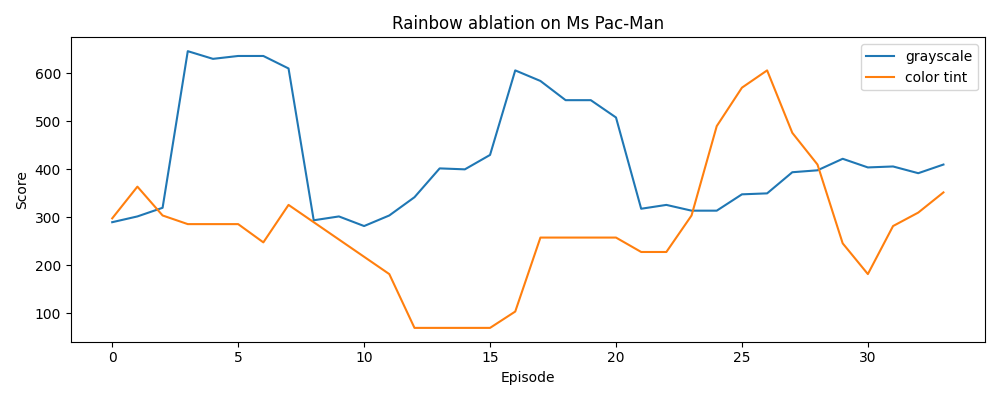
\includegraphics[width=\linewidth]{color_robustness.png}
%     \caption{Performance of Rainbow DQN under color perturbation. The model was trained on grayscale frames and evaluated in a color-tinted environment without further training.}
%     \label{fig:color_robustness}
% \end{figure}

% \subsubsection*{Implications}

% This experiment highlights a key limitation in vision-based RL: agents often fail to generalize across visually altered domains, even when the task dynamics are preserved. The reliance on pixel-level features makes them vulnerable to changes in texture, brightness, or color composition. Future work could explore techniques to mitigate this sensitivity, such as domain randomization, data augmentation, or contrastive representation learning to enforce invariance to such visual shifts.

\section{Conclusion}

Across our experiments in the \texttt{MsPacman-v0} environment, Rainbow DQN demonstrated greater long-term potential compared to PPO. While both agents showed signs of early learning, Rainbow consistently reached higher peak rewards, suggesting that value-based methods — especially those enhanced with prioritized replay, multi-step returns, and noisy exploration — are more effective at discovering high-reward strategies in sparse-reward, long-horizon settings like Ms. Pac-Man.

PPO initially showed more stable performance but suffered from later instability and reward collapse, highlighting the sensitivity of policy gradient methods to hyperparameter tuning and on-policy sampling noise. Meanwhile, Rainbow’s higher variance points to its own limitations, such as the need for more careful reward shaping or extended training to achieve consistent convergence. Nevertheless, under our limited frame budget, Rainbow's sample efficiency and reward potential clearly outpaced PPO.

\subsection{Future Work}
Other interesting things that could be tried for both our PPO and Rainbow agents in Ms. Pac-Man, we suggest three next steps. First, adding memory (LSTM) to PPO would help the agent remember past states, which is crucial for navigating mazes. Second, training both algorithms much longer—for tens of millions of frames—could help them reach superhuman scores, like top RL systems do in other games. Finally, running each experiment at least 5 times would make the results more reliable, since deep RL training can vary a lot between runs. These changes would help us build stronger agents and better understand how to master complex games like Ms. Pac-Man.

\appendix
\section{Appendix}
\label{sec:appendix}

\subsection{PPO Hyperparameter Sweeps}
\begin{figure}[H]
  \centering
  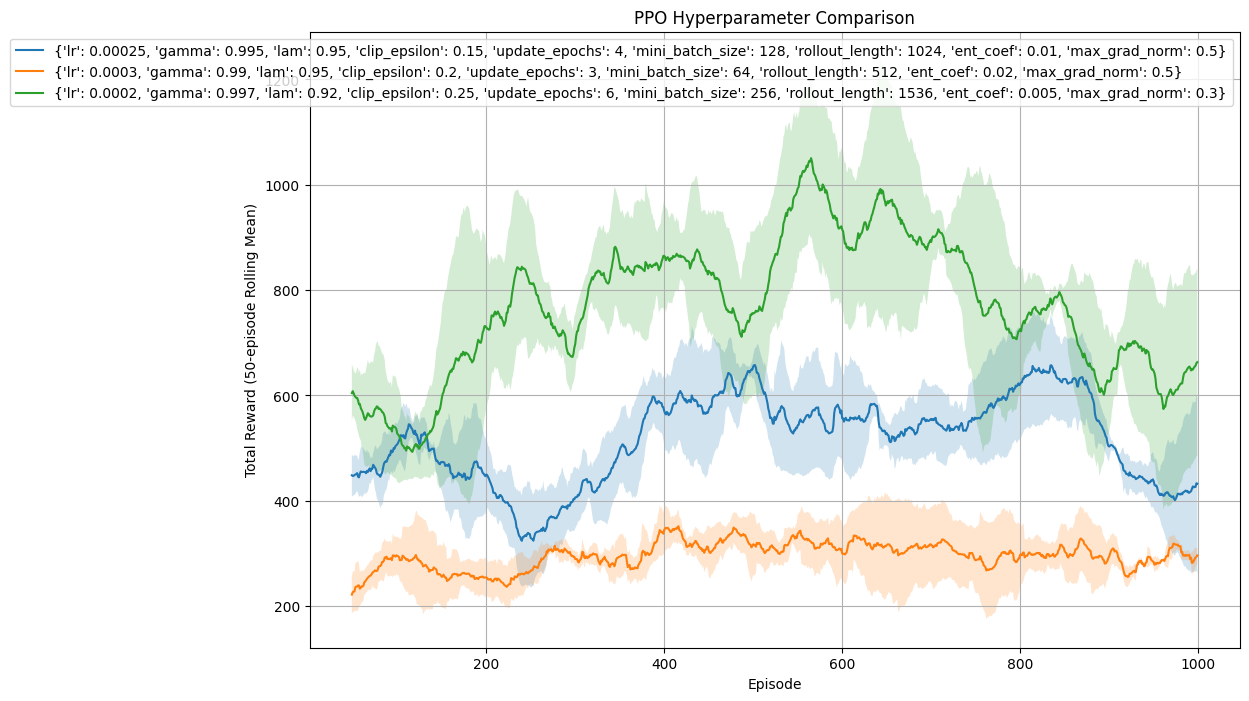
\includegraphics[width=\linewidth]{PPO_output_hyperparameters_3set.png}
  \caption{PPO Hyperparameters Optimization Results}
  \label{fig:ppo_hyperparams}
\end{figure}

\subsection{Rainbow DQN vs PPO}
\begin{figure}[H]
  \centering
  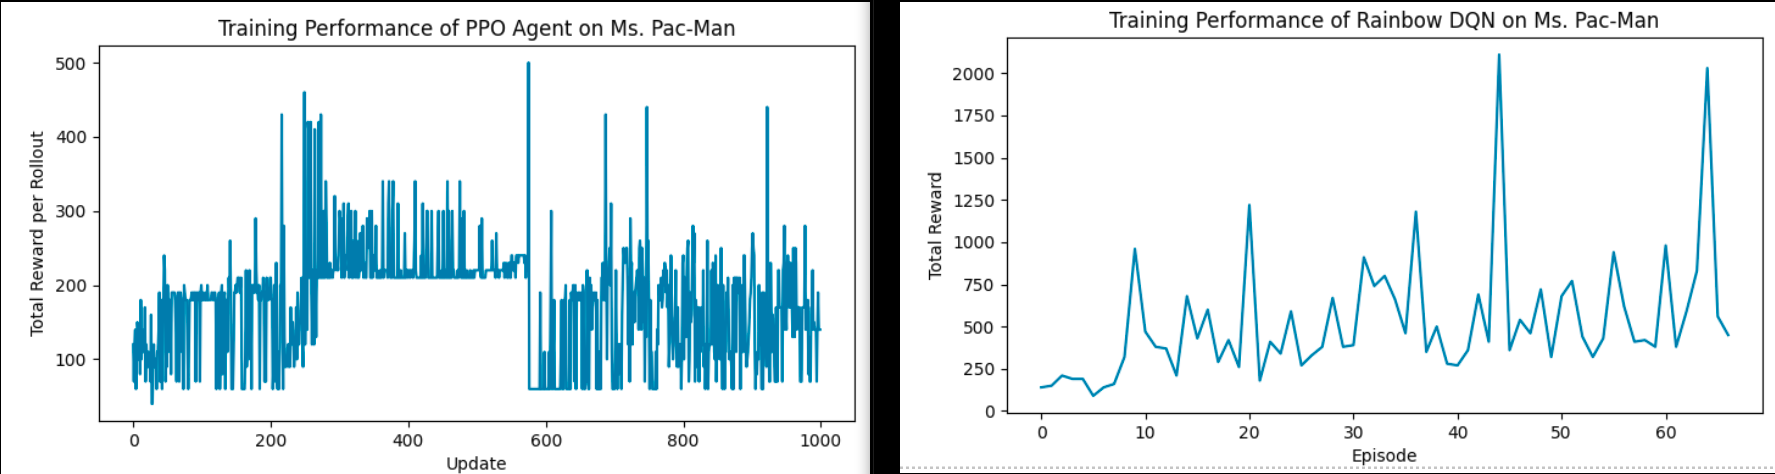
\includegraphics[width=0.85\linewidth]{rainbow_vs_ppo.png}
  \caption{Training performance of PPO and Rainbow DQN agents.}
  \label{fig:ppo_vs_rainbow}
\end{figure}

\subsection{Rainbow DQN Ablation Results}
\begin{figure}[H]
  \centering
  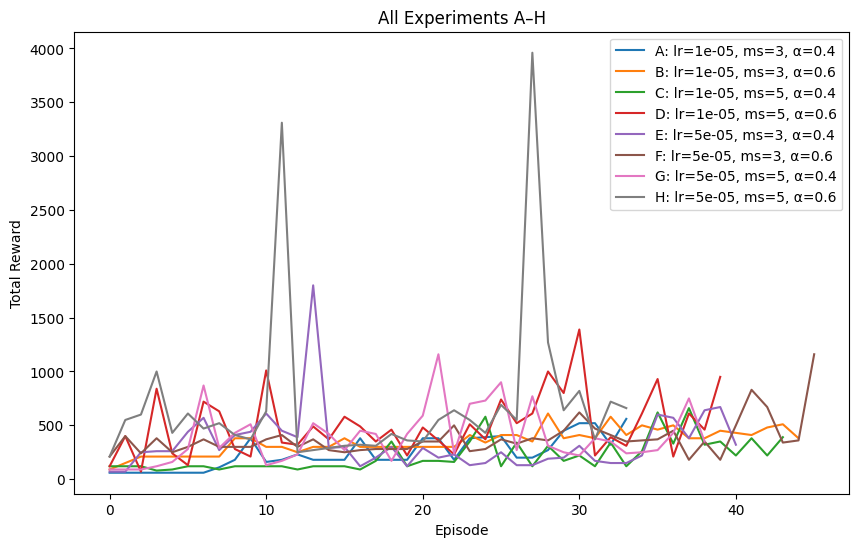
\includegraphics[width=0.8\linewidth]{rainbow_8Regular.png}
  \caption{Learning curves for the eight hyperparameter configurations:
           \(\eta\in\{1\times10^{-5},5\times10^{-5}\}\), 
           \(n\in\{3,5\}\), 
           \(\alpha\in\{0.4,0.6\}\).}
  \label{fig:ablation}
\end{figure}

\subsection{Extended Hyperparameter Sweep}
\begin{figure}[H]
  \centering
  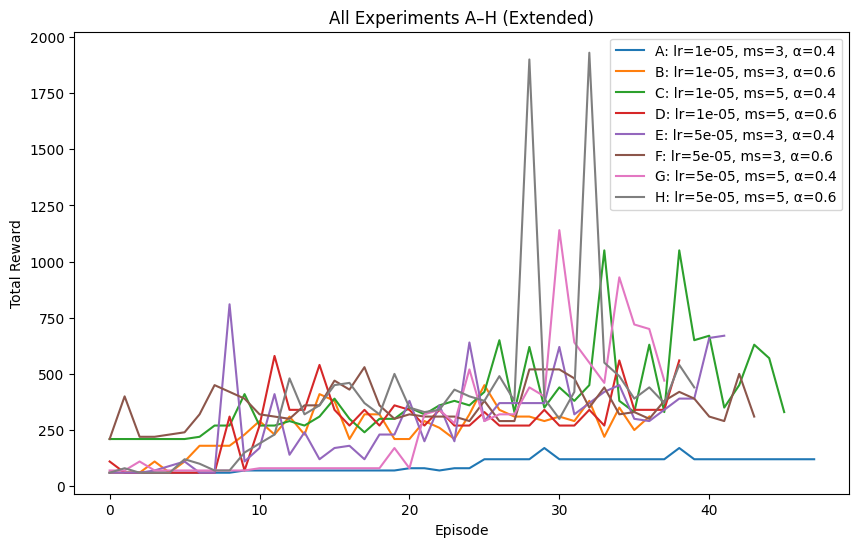
\includegraphics[width=0.9\linewidth]{rainbow_8Extended.png}
  \caption{Learning curves for the eight “large” hyperparameter runs (A\_large–H\_large).}
  \label{fig:extended_sweep}
\end{figure}

\subsection{Seed-Level Reproducibility}
\begin{figure}[H]
  \centering
  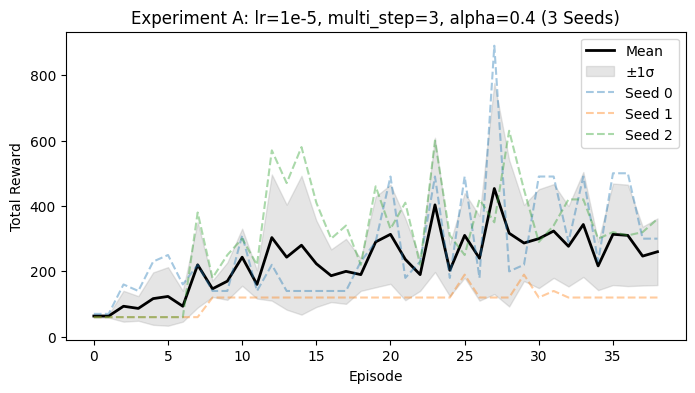
\includegraphics[width=0.8\linewidth]{rainbow_A_seed.png}
  \caption{Configuration A (\(\eta=1\times10^{-5},\,n=3,\,\alpha=0.4\)) across three seeds.}
  \label{fig:seed_A}
\end{figure}

\begin{figure}[H]
  \centering
  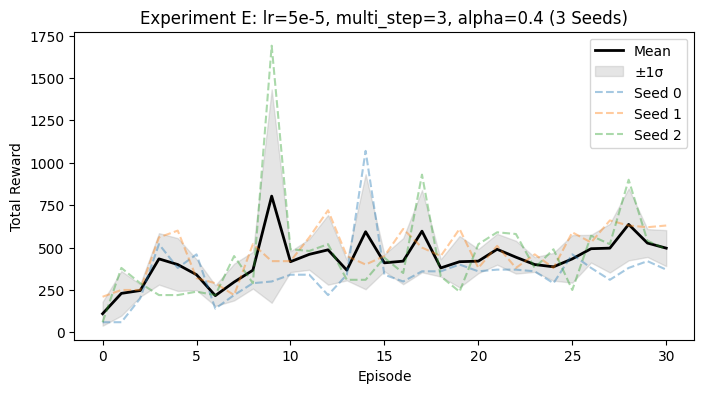
\includegraphics[width=0.8\linewidth]{rainbow_E_Seed.png}
  \caption{Configuration E (\(\eta=5\times10^{-5},\,n=3,\,\alpha=0.4\)) across three seeds.}
  \label{fig:seed_E}
\end{figure}

\subsection{Ablated Rainbow DQN Variants}
\begin{figure}[H]
  \centering
  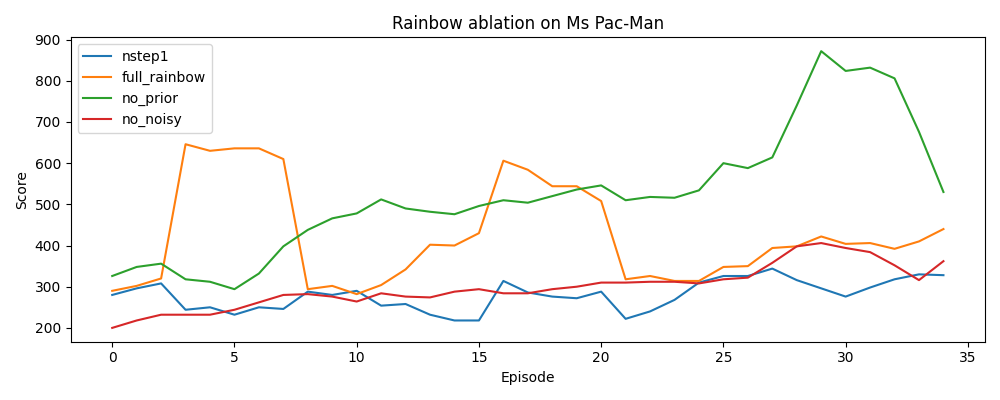
\includegraphics[width=\linewidth]{rainbow_ablation_smooth.png}
  \caption{Training performance of Rainbow DQN and ablated variants on Ms. Pac-Man.}
  \label{fig:rainbow_ablation}
\end{figure}

\clearpage
\addcontentsline{toc}{section}{References}
\bibliographystyle{plain}
\bibliography{references}

\end{document}
